
\chapter{Conclusions and Future Work}


\section{Conclusions}

In order find alternative materials to supersede superalloys, ceramics and intermetallics have been explored over the last five decades.  No viable system has been found yet, as the intrinsic low room temperature fracture-toughness of ceramics and intermetallics has to be resolved.

Ceramics offer significantly greater high-temperature advantages over superalloys than intermetallics.  The research in ceramic-matrix composites is making strides in increasing systemic fracture-toughness. 
Of the intermetallic systems being looked at, silicides have received a lot of attention.  Alloys from the molybdenum-silicon-boron system that have the solid-solution phase in equilibrium with the Mo$_5$Si$_3$ silicide and the Mo$_5$Si$_2$B T$_2$ phase display adequate fracture-toughness and good creep resistance at temperatures of up to 1500\celsius.  They also display adequate oxidation resistance in preliminary oxidation tests at intermediate and high temperatures.  Bond coat systems for protection against oxidation have recently been designed for these alloys and are undergoing further testing. 

Ultimately, in order to understand how to construct a sensible approach to intermetallic alloy design, we have to look at what strategy should be employed for the most efficient gains in relevant knowledge.  What would be an appropriate definition of efficient?  A first approximation could be: the collection of salient knowledge.  What are the potential deal-breakers?  We could define deal-breaker as any property that would prevent alloy implementation in the hot section of jet-engines.  Given that several potential deal-breakers had been identified, these needed to be sensibly ranked in order to proceed with an effective strategy.  Resources had be allocated to determine if these potential deal-breakers exist on the physical plane.  If the highest ranked deal-breaker does not exist, hurrah.  We can then move down the list and determine if the next-highest-ranked deal-breaker exists.  If it does, we could then determine whether it can be circumvented through exploration of alternative solutions.   In this project, we principally want to find out whether these eutectic alloys have the potential to be mechanically superior to superalloys.  We have defined `mechanically superior' as `being substantially stronger than superalloys at 1200\celsius'.  Secondly, we have established that some of the alloys in the systems explored would not ``pest" as badly as Mo and Nb alloys, but have poorer oxidation properties than superalloys.  Extensive determination of alloy oxidation properties would not have brought clarity at this early stage.  Allocating resources to this endeavour would have been unstrategic and would have detracted the project from the most effective path of salient knowledge collection.  

%To collect ``low-lying fruit", as it were, would be detract the project from the most effective path of salient knowledge collection.  
%There is a corresponding inefficiency associated with being too curious.  Strict adherence to conventional evaluation methods used for is unwise.  
%The world is already drowning in data; data acquisition for the sake of possessing more data is unneccessary.  
%For instance, the conventional oxidation tests and analysis used for nickel-based superalloys, if applied to this project, would have been excessive.  

We still found it wise to draw from our expertise in nickel-based superalloys to construct a sensible approach to designing our first intermetallic alloy.  The distinctly novel aspect of this project was the implementation of the "Solubility Index" concept in our alloy design.  This allowed us to maximise the effects of alloying additions through the careful study of the limited phase-diagram information published, while allowing us to minimise the chances of precipitating unwanted phases that would introduce unneccessary additional variables to our analysis.
  
We have considered a number of intermetallic systems and concluded that the most promising initial step in alloy design would be to explore (Cr, V)$_{solid}$ $_{solution}$--(Cr, V)$_3$Si$_{intermetallic}$ alloys.  These two-phase eutectic alloys have a solid-solution phase for fracture-toughness and an intermetallic phase for high-temperature strength.  They have low density, and have been designed to have no phase transformation at all operating temperatures, and no precipitation of undesirable additional phases.  Chromium had been chosen as a constituent to provide oxidation and corrosion resistance to temperatures of up to 900\celsius, and silicon had been chosen to provide oxidation resistance at temperatures above 900\celsius.  Fracture-toughness issues faced by chromium include its intrinsic brittleness at room temperature and its susceptibility to embrittlement due to interstitial impurities, especially that of nitrogen-embrittlement at high temperatures.  Vanadium is ductile at room temperature, and forms a perfect solid-solution with chromium.  It was hoped that alloys containing vanadium would demonstrate an increase in fracture-toughness, partly through the intrinsic character of vanadium, and partly through a decrease in the number of ordered bonds in the solid-solution.  V$_3$Si has been reported to display higher hardness than Cr$_3$Si at all temperatures up to 1200\celsius, and can contribute high-temperature strength to the alloy system.  The lack of oxidation resistance of vanadium can be countered by keeping its content low, and maximising chromium and silicon content.

Arc-melt manufacture ingots were made to locate eutectic compositions, making arc-melt processed feed ingots for RF DS and mirror furnace casting, microstructural examination using optical microscopy and SEM, and compositional analysis using the in-house SEM and the WDS facility at the University of Edinburgh.  Large cooling stresses during arc-melting and PM manufacture caused specimen cracking and crumbling.  Alloy microstructures were not fully eutectic for several reasons.  There are probably strict composition ranges in the binaries and ternaries during rapid solidification, the very high melt viscosities experienced made homogenisation difficult, and there was insuffficient mixing in the melt with the manufactured methods pursued.  The large differential in element densities led to segregation and separation within each specimen.  Once segregation occurred, dendrite formation would be encouraged.  Once dendrites formed during solidification, it would not have been conducive for lamellar eutectic formation as the melt composition would have shifted away from the eutectic composition.  A large cooling-rate differential within each specimen resulted in dendritic microstructures in some grains and eutectics in others.  A lack of an effective means of mechanical mixing compounded the issues faced in specimen manufacture quality.  The many factors affecting microstructure made it difficult to fine-tune the compositions to achieve a fully lamellar microstructure.  The presence of intermetallic dendrites would not have improved specimen fracture-toughness.

The binary and ternary alloys were isothermally oxidised at 800\celsius\ and 1200\celsius.  None of the alloys were able to form a protective silica layer.  All V-containing alloys volatilised substantial rust-coloured vanadium pentoxide.  The ternary alloys fared better than the binary alloys.  They managed to form islands of silica crystals interspersed within a mixed (Cr, V) oxide.  ($\frac{3}{4}$Cr, $\frac{1}{4}$V)-- ($\frac{3}{4}$Cr, $\frac{1}{4}$V)$_3$Si and ($\frac{1}{2}$Cr, $\frac{1}{2}$V)-- ($\frac{1}{2}$Cr, $\frac{1}{2}$V)$_3$Si were considered to have the best oxidation resistances as they volatilised comparatively low volumes of vanadium pentoxide, and did not experience runaway oxidation or massive oxide spallation.  Based on these results, we used ($\frac{1}{2}$Cr, $\frac{1}{2}$V)-- ($\frac{1}{2}$Cr, $\frac{1}{2}$V)$_3$Si as the base alloy in our alloy design, and substituted out vanadium to make way for alloying additions.  In doing so, there is some security that the quaternary and quinary alloys will not experience runaway oxidation at intermediate and high temperatures, as the alloying additions have better oxidation properties than the vanadium being substituted out.

We also thought it sensible to compare the mechanical properties of either a bench-mark silicide alloy, or one of the alloys designed, when manufactured through both directional solidified and hot isostatic press processing of powder.  This allows us to determine the superior route for obtaining optimised mechanical properties.  The fine microstructure of powder-HIPped manufactured material has been shown to be effective at partitioning load.  Additionally, chromium has been reported to be susceptible to heavily exothermic reactions when combining with other alloying elements, to be prone to cracking during casting, and brittle.  It has not been found to be castable on a large scale.  This is why alloys with high chromium content are typically powder-HIPped processed.  Nevertheless, it was the opinion that an alloy that had been very slowly cast using DS manufacture may be able to overcome the issues a conventionally cast alloy would face.  It would have a lamellar microstructure which may improve fracture-toughness by increasing critical crack length through crack-deflection.  A microstructure with its intermetallic phase aligned along the loading axis may be effective at withstanding load.  

Due to limited funds and equipment access, alloys could only be DS manufactured and not powder-HIPped processed.  Directional solidification manufactured ingots had better fracture-toughness than their arc-melt or PM manufacture counterparts.  They did not break into several pieces upon cooling down from solidification temperature, and did not break when lightly tapped with a hammer to break them out of their ceramic crucibles. 

Microstructure examination showed formation of dendrites in all samples.  High melt viscosity and poor melt-mixing were clearly still issues in DS manufacture, especially for the ingots with high chromium and tantalum content.  In \ilovewill{山}Ta, the presence of dendrites of both solid-solution and intermetallic phases show the extensive influence that viscosity and lack of mechanical mixing have on the solidification front.

Efforts required to optimise the manufacturing process of such high-temperature materials must not be underestimated.  If one’s alloy manufacturing process produces samples of poor quality, any mechanical testing will only define the properties stemming from the samples’ weaknesses and inhomogenieties.  True alloy properties will not be realised. 

It may be said that one should address the cause of the high differential of cooling rates rather than making attempts to circumvent it.  Samples with such differentials will experience cracking during manufacture or machining, and cannot be used in mechanical testing of any sensible form.  In order to improve the machinability and fracture-toughness of the silicide alloys, they must be cooled very slowly past their DBTT during manufacture.  Rates of 5\celsius/minute or lower would be ideal.  This way, internal strains due to the differential in phase CTEs will be minimised, if generated at all.

The X--X$_3$Si eutectics, when slowly directional-solidification manufactured, form a very coarse lamellar microstructure, with the intermetallic precipitates growing along the loading axis.  It would seem that a lamellar microstructure with a coarse inter-lamellar spacing of 5\micro\metre\ does not allow for effective load-partitioning.  A smaller inter-lamellar spacing is required to impede dislocation motion, increase constraint effects and thus increase high-temperature strength.  This can be produced using powder metallurgy or through rapid solidification rates.

Despite concerted and protracted efforts to facilitate successful high-temperature tensile-testing, we were not able to obtain any sensible data due to samples of insufficient quality and lack of adequate testing facilities.  Through the tensile tests conducted in-house and at ENGINX, all alloys were found to have DBTTs of higher than the facility's maximum operating temperature of 1000\celsius.  Samples would experience brittle fracture long before their elastic limits were reached.  Brittle fracture could be circumvented by testing at a temperature above DBTT, but this was not possible due to the absence of access to appropriate equipment in Europe.  With the seemingly insurmountable troubles encountered in DS ingot manufacture, we strongly suspected that powder-HIPped specimen manufacture would prove to be more sensible.  At this stage, we had worked on the project for over a year, did not have money or equipment for powder-HIP manufacture, and realised that we had to work with what we had or abandon the project.

The opportunity to properly test specimens at high temperature was finally feasible in the last month of the project's 3$^{rd}$ year, using Professor Kumar's bespoke ultra-high-temperature facility at the Engineering Department of Brown University.  This was a one-off situation, and the relatively short time allocated meant that tensile testing had to be sacrificed to ensure that sufficient time was available to collect compression data across all the relevant alloys.  We were able to show that \ilovewill{山}, \ilovewill{山}W, \ilovewill{山}Ta and \ilovewill{山}TaAl had better compression properties than superalloys at 1200\celsius.  Alas, high-temperature compressive strength is not a property that is sought after in blade alloys.

The base alloy, \ilovewill{山}, is stronger than the binaries at 1200\celsius\ and 10$^{-4}$/s.  10$^{-4}$/s tests at 1200\celsius\ and 1300\celsius\ to ascertain improvements in mechanical behaviour due to Ta additions are inconclusive.  \ilovewill{山}TaAl is the strongest lamellar alloy at 1300\celsius.  \ilovewill{山}W had the best compressive properties at 1200\celsius\ and 1300\celsius\ by at least an order of magnitude.  When compared to the high-temperature compression and compression-creep testing of HIP manufactured Mo- and Nb- containing alloys at Brown University, the DS manufactured eutectics explored display inferior high-temperature properties with differences quantifiable in orders of magnitude.

%
\begin{figure}[H]
\begin{center}
\includegraphics[width=16cm]{flow}
\caption{Schematic of alloy development in this project.}
\label{fig:flow}
\end{center}
\end{figure}
%

No tertiary phases precipitated in any of the ternary alloys.  The binaries and ternaries all had two-phase lamellar structure, with the high Cr-content alloys forming a finer, more ordered microstructure (Figure \ref{fig:flow}).  The ternaries performed better than the binaries in compression at 1200\celsius.  Many iterations were required to manufacture specimens without extensive dendritic regions.

The quaternary addition of Ta to \ilovewill{山} resulted in the formation of two distinct populations of eutectic cells, but did not destabilise them (Figure \ref{fig:flow}). No tertiary phases formed.  High melt viscosity, poor melt-mixing, and a probable complicated solidification path induced segregation to such an extent that two primary dendrites of both phases grew adjacent to each other throughout every specimen.  When tested at high temperature, it exhibited strength that was inconsistent.  This was found to be due to gross specimen inhomogeniety; one sample contained no Ta.  It is believed that if specimens close to nominal composition were manufactured, they would exhibit mechanical properties that are on par with \ilovewill{山}TaAl.
 
The quinary addition of Al to \ilovewill{山}Ta decreased melt viscosity, which allowed for greater sample homogeniety.  Al did not destabilise or coarsen the lamellar structure; it did, however, create two populations of solid-solution. This was seen in the quantitative area maps acquired through WDS.  The aluminide existed as two populations that had distinct, but very similar, chemical compositions.  This alloy had a very complex microstructure.  It was surprisingly tough and not prone to cracking during machining.  Although the addition of Al liquidised the melt, this probably diminished the alloy's high-temperature structural properties.  Al and its aluminides are known to be structurally weak at high temperatures.  As no valid data is available for \ilovewill{山}Ta for direct comparison with \ilovewill{山}TaAl, we cannot ascertain the effect of Al.

Quaternary \ilovewill{山}W had a coarse and grossly degenerate microstructure with hardly any lamellar microstructure.  Its chemical components were X$_3$Si and solid-solution.  When compressed at 1200\celsius and 1300\celsius, it was incredibly strong and we could not put it into its plastic regime using the 5kN stress-rig.  These results are counter-intuitive, given that its microstructure was so coarse.  The high Si content in its solid-solution probably strongly contributed to these structural properties.  From this, it can be seen that the effects of chemistry can outweigh the effects of an optimised microstructure.

The addition of Al to \ilovewill{山}W formed quinary \ilovewill{山}WAl (Figure \ref{fig:flow}).  \ilovewill{山}WAl  had a coarse microstructure that was very similar to quartenary \ilovewill{山}W.  It had a solid-solution phase and an X$_3$Si intermetallic phase.  It had very poor mechanical properties that were worse than the ternaries, quaternaries, the other quinary, and the Cr--Cr$_3$Si binary.  It performed only slightly better than the V--V$_3$Si binary.

%fracture-toughness of all specimens.
% handling
%cracked during processing?
%pesky handling

The fantastic creep performance of negatively-misfitting superalloys at 1100\celsius, a temperature very close to their homologous temperatures, is partly due to the rafts that form.  When superalloys of negative misfit raft, each raft is a large thin plate.  Dislocations are for the large part unable to travel further when they hit a raft of $\gamma$'.  When superalloys with a positive misfit raft, they form rods. Horizontal $\gamma$ channels weld together due to the load symmetry, and the two orientations of vertical channels remain unrafted and open.  At high temperature, when a dislocation travels through the ductile $\gamma$ solid-solution and impinges upon a rod, it is able to bow around the intermetallic rod quite easily.  This mechanism is conducive for creep.  Negatively-misfitting alloys thus demonstrate superior high-temperature tensile properties.

It is unfortunate that the DS manufactured eutectics explored do not form fine, plate-like, lamellar microstructures.  The slip systems which are most highly stressed make angles close to 45$\degree$ to the tensile axis, and a plate-like microstructure aligned either perpendicularly or normal to the loading axis would be effective at halting dislocation motion at high temperature.  Instead, due to their globular and undisciplined nature, these alloys experience predominantly solid-solution plastic flow, and the intermetallic phase is unable to take up the load effectively.
 
The analogies drawn between nickel-base superalloys and DS eutectics in this work have been shown to be limited and superficial.  The structural performance of any peak-aged two-phase nickel-based superalloy is greater than the sum of its parts.  DS manufactured X--X$_3$Si eutectics deform by solid-solution plastic flow and are weaker than the sum of the constituent phases.  Why is this the case?

It has often been said that the structural properties of superalloys stems from $\gamma$' ability to maintain a fine, coherent, and hence stable array of precipitates.  This coherency is due to the similar crystal structures of FCC Ni solid-solution and L1$_2$ Ni$_3$Al.  Dislocations get drawn into the fine $\gamma$' precipitates, and because of the occurrence of anomalous hardening, this array is able to ``resist the intrusion of single dislocations and impede the ingress of paired dislocations" ~\cite{cathie12}.  This, however, is an unsatisfactory explanation, as it does not detail the impediment of intrusion and ingress.  

In a single-phase $\gamma$' alloy made to replicate the composition of Nimonic 105's $\gamma$' phase, peak strength occurs at a low temperature of 600K in the [111] orientation (Figure \ref{fig:anomalous}) ~\cite{nembach00}.  At temperatures above 600K, $\gamma$ experiences a drop in strength because its dominant deformation mechanism switches from octahedral glide to cube-slip.  If the stress-axis is [001], there will be zero resolved shear stress on the cube-slip planes.  The plane perpendicular to applied stress has no stress acting on the dislocations.  Vertical channels, although parallel to applied stress and possess Burgers vectors, have plane areas that are essentially infinite.  The two-phase superalloy, however, shows excellent flow stress in both the [111] and [001] orientations up to 1100K, which is the temperature of $\gamma$' dissolution.  Cube-slip does not occur in the disordered solid-solution.  Peak-aged precipitates are thus `` large enough to allow the cross-slip of the dislocation pairs to add to the flow stress and produce the anisotropy observed, but small enough for those sections of the dislocations in the matrix to constrain the flow on to the octahedral planes" ~\cite{cathie12}.  In the two-phase $\gamma$/$\gamma$' alloy, dislocations are essentially  lured into $\gamma$' and find themselves trapped in the quagmire of anomalous hardening.

Unlike superalloys, DS manufactured X--X$_3$Si eutectics are much more akin to a composite system.  The solid-solution and intermetallic are incoherent, and there is a lack of coupling between the the two phases.  They are essentially two different structures with very different Burgers vectors.  Hence, despite the orientation relationship between the solid-solution and X$_3$Si, this is not sufficient to ensure continuity of slip.  Dislocations find it easy to travel in the coarse solid-solution and are generally unable to enter the intermetallic phase to allow it to bear some of the load at high temperature.  As a consequence, they possess poorer structural performance. 

It would be ideal to use powder metallurgy to manufacture the base alloy \ilovewill{山}, the quaternaries and quinaries to see how their mechanical properties would compare with both their DS counterparts, and Mo- and Nb-silicides.

The progress of good science need not be a protracted struggle.  When an ambitious, novel project is undertaken, access to a modicum of common sense, a proper manufacturing route, and an appropriate test-rig, are non-negotiable.  Otherwise, one's efforts could be said to be for naught.  Being able to achieve project goals and being able to acquire data precision can be muddled together like mint and rum, but one should not make the mistake of equating accurate data with the right answer.  Perhaps Richard Feynman sums it up best in his concluding paragraph in the Challenger report: ``For a successful technology, reality must take precedence over public relations, for nature cannot be fooled."

To employ a strategy of circumvention of the key issues faced in intermetallic alloy design is to employ a suboptimal approach.  It is cop-out.  In order to implement disruptive technology, an equivalent incremental benefit would need to result in order to justify the high costs involved during implementation.  It may be that silicides will find usage in niche applications.  At present, it seems unlikely that large-scale implementation in aeroengines would be economically feasible.

 

\section{Future Work}

HIP manufacture using powder and high-temperature testing of \ilovewill{山}, the quaternary and the quinary alloys will allow us to determine whether HIP or DS manufacture produces superior properties.  From this, we will also be able to estimate how the (Cr, V) X--X$_3$Si properties are relative to the (Mo, Nb) X--X$_5$Si$_3$ and X--X$_5$Si$_3$--T$_2$ alloys.

In Subsection 3.6.1, Mo$_5$SiB$_2$, a T$_2$ phase (Figure \ref{fig:T2structure}), was described to be an extremely creep resistant phase at high temperature ~\cite{rawn01}.  Incorporating it can allow for improvements in creep properties, in addition to widening the number of phases that can be formed in the system.  Chromium additions would destabilise the T$_2$ phase, as seen in Figure \ref{fig:CrSiB}.  This phase forms via a peritectic reaction, and would require further alloying additions to either tease it into a eutectic reaction ~\cite{sakidja05}, or to counter Cr's T$_2$ phase de-stabilization ~\cite{nowotny58}. 

There is no ternary phase-diagram available for the V--Si--B system except for the schematic drawn by Sakidja and Perepezko (Figure \ref{fig:T2_alloying}) ~\cite{sakidja05}.  The analogous V$_5$SiB$_2$ has been reported.  An approach to incorporate T$_2$ into the X--X$_3$Si eutectic structure would be to ascertain if a X--X$_3$Si--X$_5$SiB$_2$ eutectic occurs in this system. 

Chromium substitutions of vanadium could be made to investigate the extent of ternary eutectic destabilisation.  The threshold of chromium concentration at which the X$_5$SiB$_2$ phase becomes destabilised in the (Cr, V)--(Cr, V)$_3$Si--(Cr, V)$_5$SiB$_2$ ternary eutectic could be assessed.  The eutectic could then be extended to (Cr, Mo,V)--(Cr, Mo,V)$_3$Si--(Cr, Mo,V)$_5$SiB$_2$.  Mo additions can further stabilise the T$_2$ phase.  Rawn reports that B substitutes for Si to a limited extent in the Mo--Si--B system.  This suggests that the composition of T$_2$ is not necessarily stiochiometric.  If the ternary V--Si--B system were expanded to include more elements, we might find that this B--Si ratio may change.

Finally, it is clear that any future work must have access to adequate facilities for specimen manufacture of samples with the appropriate fine microstructure. This fine microstructure may be directional.  Since such work is focussed on finding alloys that can operate at temperatures in excess of 1100\celsius, salient property assessment must include high-temperature mechanical testing.

%
\vspace{2cm}
\begin{figure}[H]
\begin{center}
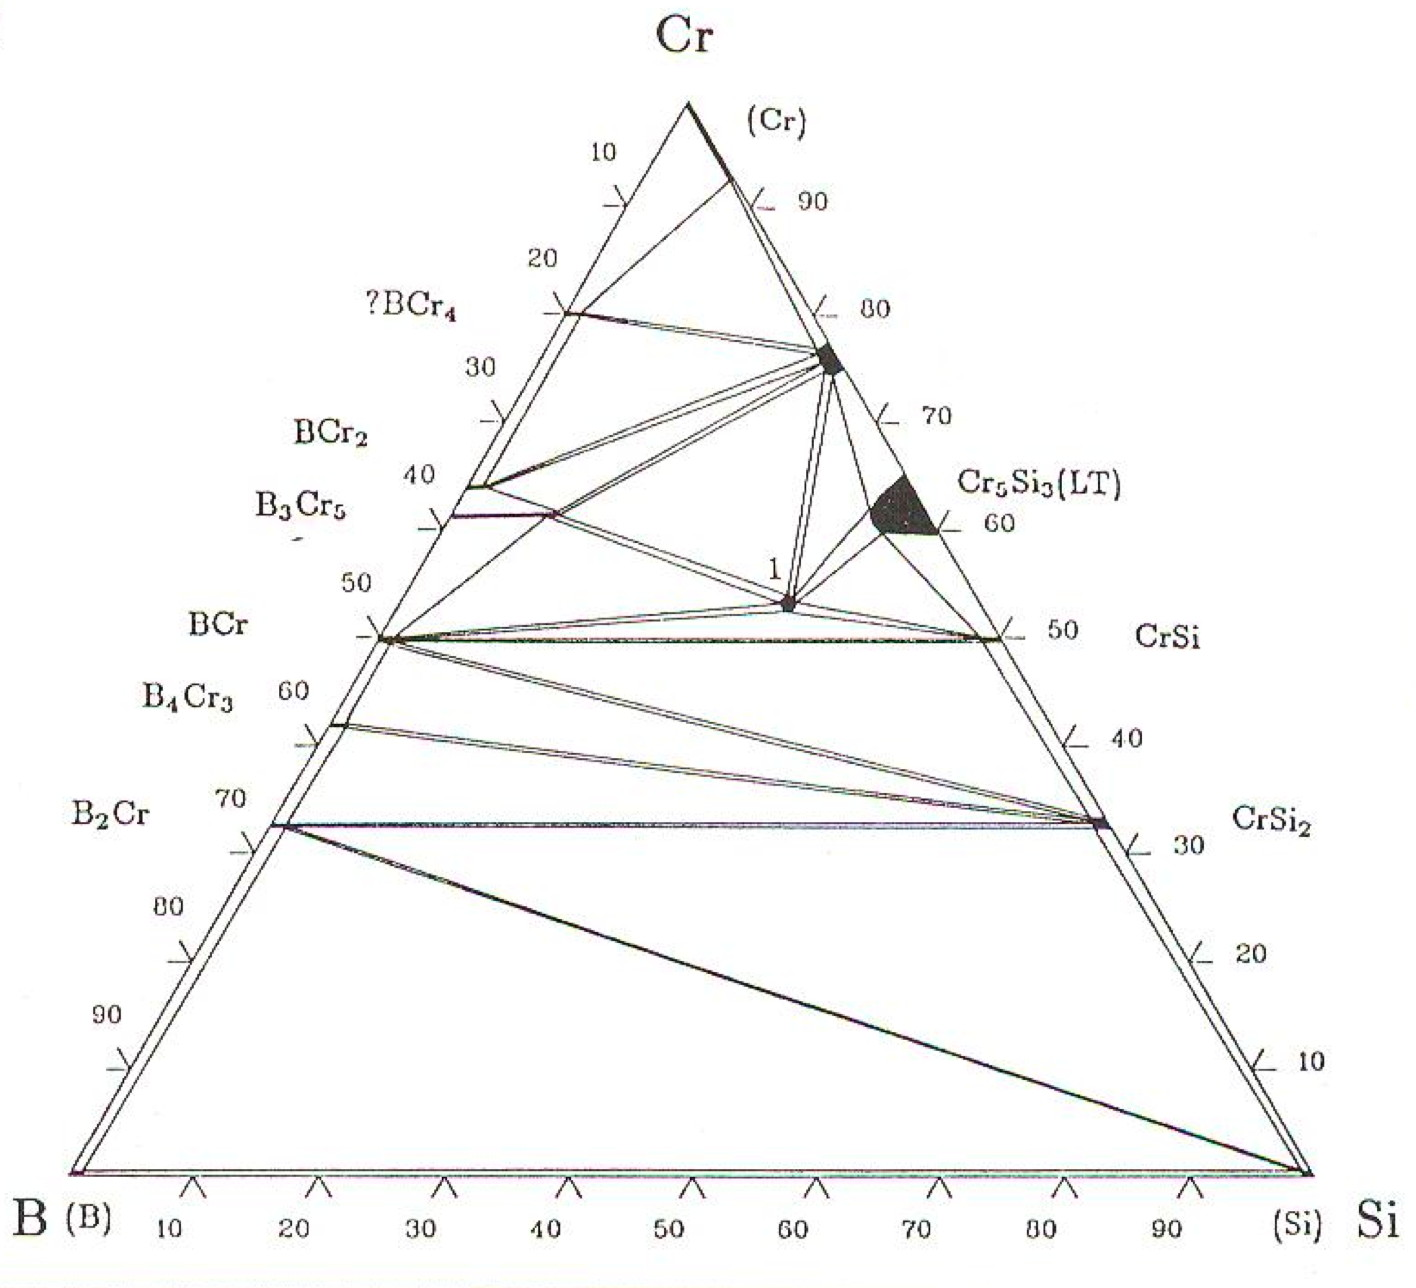
\includegraphics[width=\textwidth]{CrSiB}
\caption{Ternary phase-diagram of Cr--Si--B ~\cite{nowotny58}.}
\label{fig:CrSiB}
\end{center}
\end{figure}
%
\begin{figure}[H]
\begin{center}
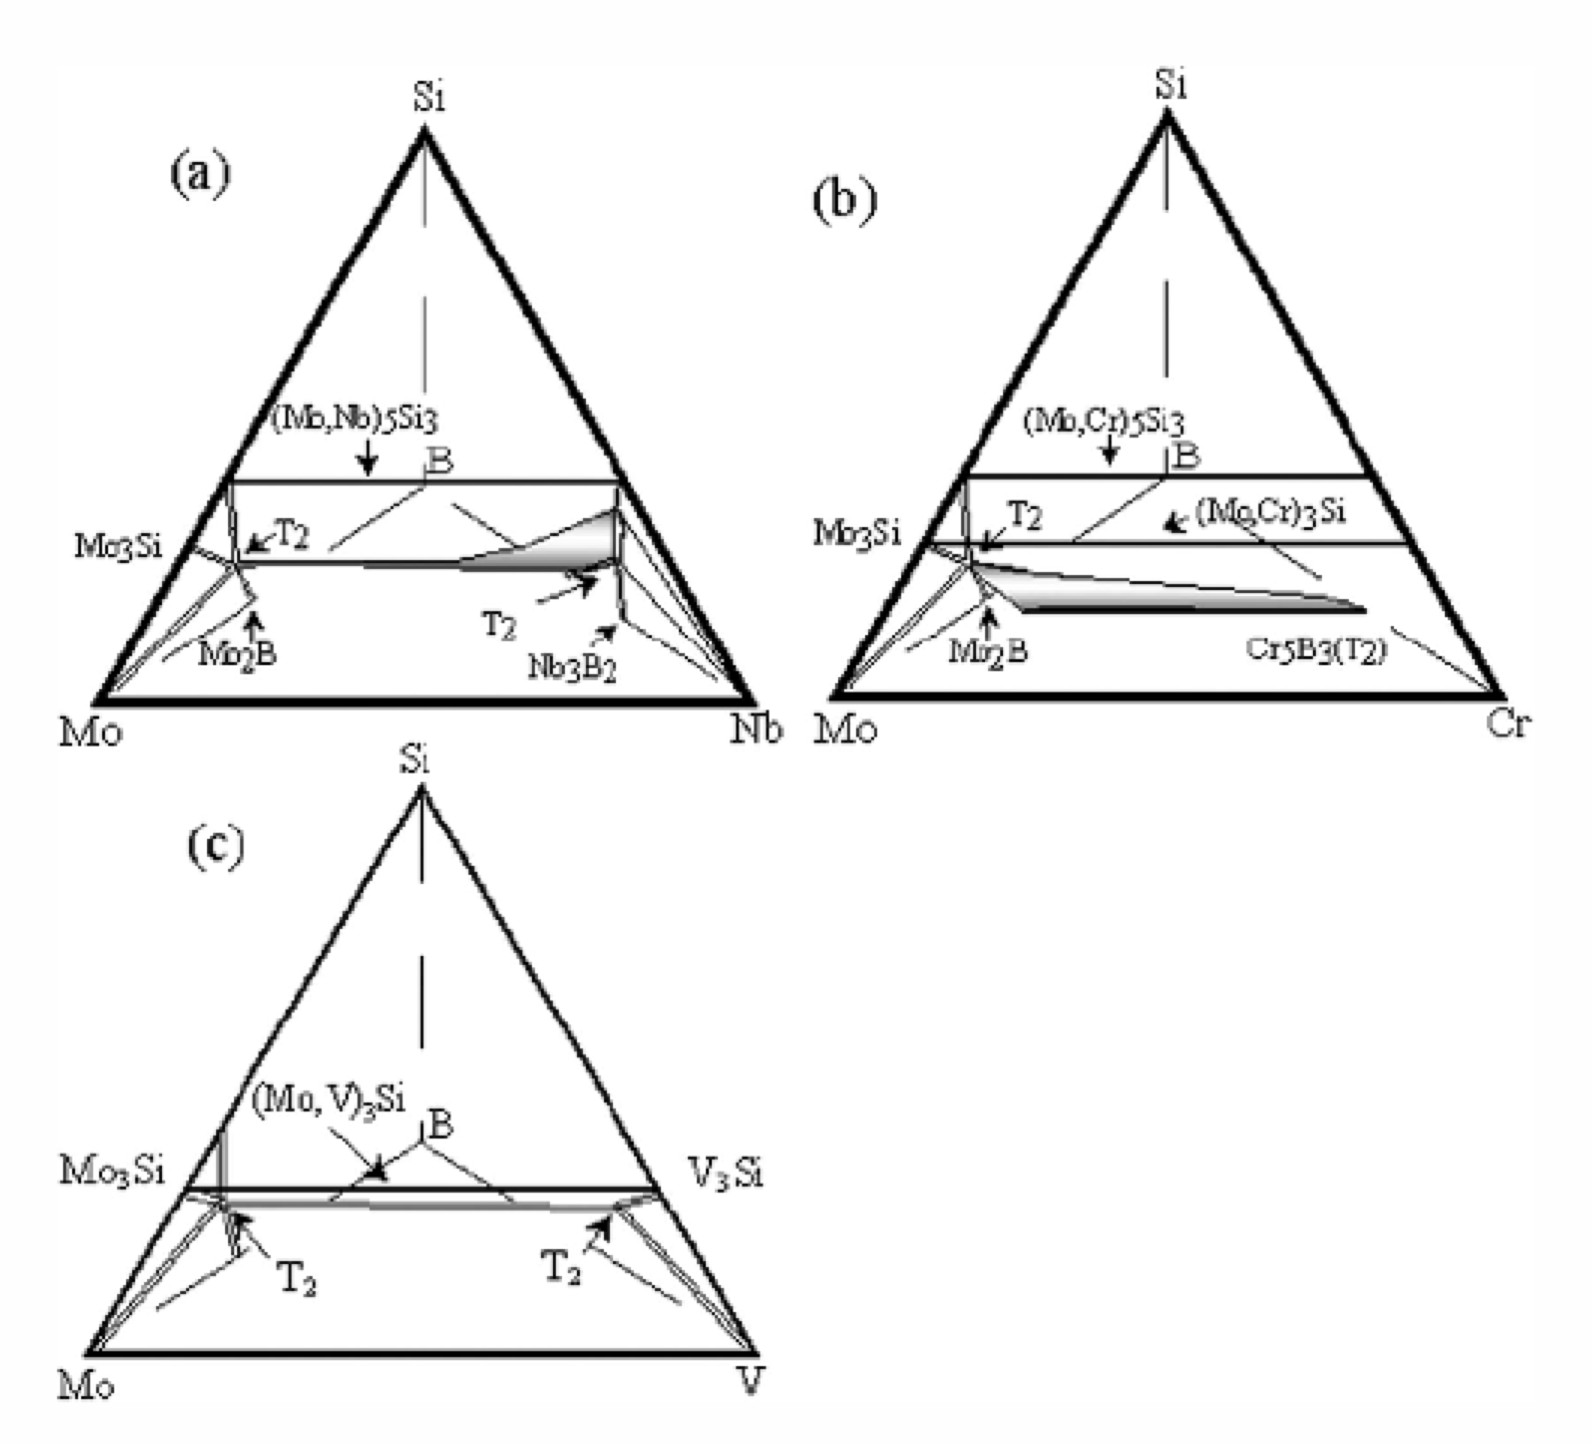
\includegraphics[width=\textwidth]{T2_alloying}
\caption{Schematic illustration of observed solubility for selected transition metal (TM) substitutions in both the bcc and the T$_2$ phase in the quaternary Mo--TM--Si--B. ~\cite{sakidja05}.}
\label{fig:T2_alloying}
\end{center}
\end{figure}
\vspace{-.5cm}
%
